\chapter{Komplexe Zahlen}



	\section{Einf"uhrung}
\underline{Problem:} Es gibt algebraische Gleichungen, die in der Menge  der reellen Zahlen $\R$  keine L"osung besitzen.\\
\\
$\Rightarrow x^2 + 1 = 0   $\\
$\Leftrightarrow x = ± \sqrt{-1}$ Keine Reelle L"osung!\\
\\
Es kann hierbei ein neues Symbol eingeführt werden : $i = \sqrt{-1} $\\
Damit kann man der obigen Gleichung die Lösung $x =±i$ zuordnen\\
\\
Wenn wir voraussetzen, dass diese neue Zahlen nach denselben Rechengesetzen genügen, wie die reellen Zahlen, erhalten wir damit auch Lösungen für andere bisher nicht lösbare quadratische Gleichungen, wie das folgende Beispiel zeigt:\\
\\
$\Rightarrow x^2 + 2x + 5 = 0$\\
\\
$\Rightarrow x = \dfrac { -2± \overbrace{ \sqrt{4-20}}^{=\sqrt{16*(-1)}} } { 2}
=\frac {-2 ±4i}{2}
= -1±2i$\\
\\
\\
\begin{Bemerkung}
Bezeichnungen\\
\end{Bemerkung}

\begin{enumerate}
\item Der Ausdruck $\sqrt{-1}$ heißt \textbf{imaginäre Einheit} und wird hier mit $i$ bezeichnet.
\item Ausdr"ucke der Form $i\cdot y$ mit $y \in \R$  heißen \textbf{imagin"are Zahlen}
\item Ausdr"ucke der Form $z =x+i*y$ mit $x,y \in \R$ werden als \textbf{Komplexe Zahlen} bezeichnet
\item Ist $z =x+i*y$ eine Komplexe Zahl, so heißen\\
\indent $x=Re(z)$ \textbf{Realteil} von $z$\\
\indent $y=Im(z)$ \textbf{Imaginärteil} von $z$
\item Die Menge $\C =\{ {z = x+j y| x, y \in \R}\}$ wird als Menge der Komplexen Zahlen bezeichnet\\
\end{enumerate}

\begin{Bemerkung}
Aber\\
\end{Bemerkung}

Der  \textbf{Imaginärteil} $y$ einer komplexen Zahl  $z =x+i*y$ ist selbst eine reelle Zahl! Der \textbf{Imaginärteil} ist lediglich der Faktor bei $i$!\\

	\section{Darstellung komplexer Zahlen}

Eine komplexe Zahl wird durch zwei reelle Zahlen charakterisiert. Wie bei zweidimensionalen Vektoren brauchen wir hier zur geometrischen Veranschaulichung auch eine zweidimensionale Ebene.\\

	\subsection{Kartesische Darstellung}

Jeder komplexen Zahl $z =x+i*y$ entspricht genau ein Punkt $P =(x,y)$ in der komplexen Zahlenebene und umgekehrt.\\

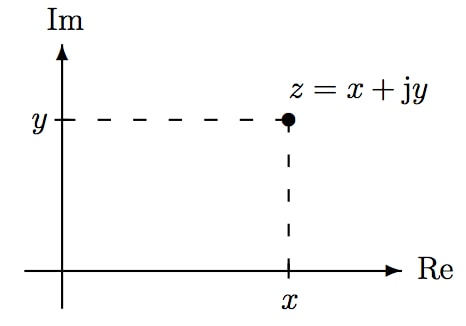
\includegraphics[width=3in]{kap6/komplexezahlen1}

\begin{Bemerkung}
Bezeichnungen\\
\end{Bemerkung}

\begin{enumerate}
\item Die komplexe Zahlenebene nennt sich auch Gaußsche- Zahlenebene
\item Hier werden die Achsen des Koordinatensystems als \textbf{reelle Achse} bzw. \textbf{imagin"are Achse} bezeichnet.\\
\end{enumerate}

\begin{Bemerkung}
Beispiel\\
\end{Bemerkung}

Die folgenden komplexen Zahlen sind in der Gaußschen Zahlenebene darzustellen: \\
$z_{1} = 2+3*j$  $z_{2} =-3-j$ ($i$ wird hier $j$ genannt)

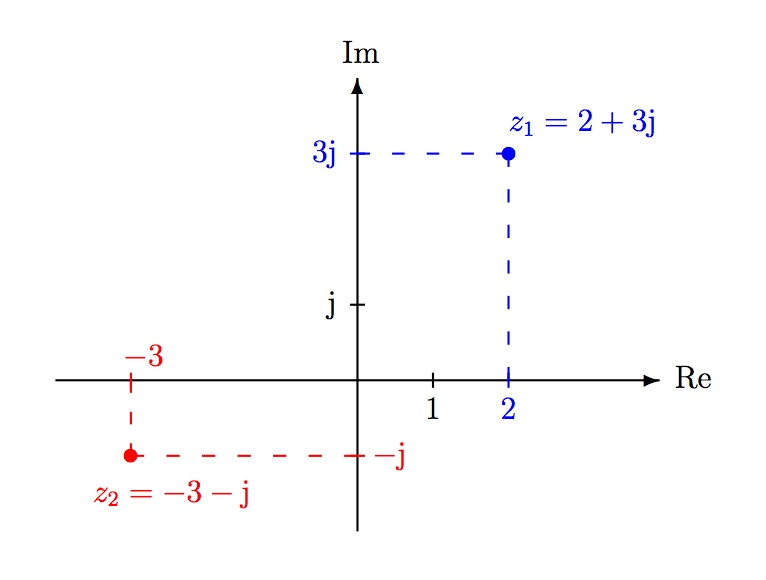
\includegraphics[width=3in]{kap6/komplexezahlen2}

\begin{Bemerkung}
Bemerkungen\\
\end{Bemerkung}

F"ur manche Anwendungen ist es hilfreich, eine komplexe Zahl nicht als Punkt $P=(x,y)$ in der Gaußschen Zahlenebene zu veranschaulichen, sondern stattdessen den Ortsvektor zu betrachten

$z=x+j*y \Leftrightarrow z=
\begin{pmatrix}
x\\
y\\
\end{pmatrix}$

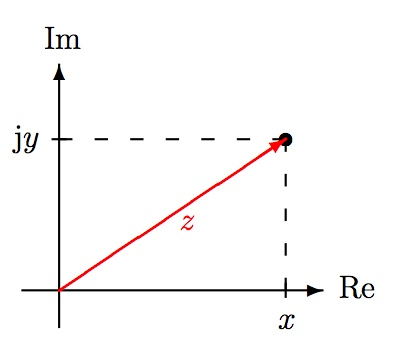
\includegraphics[width=3in]{kap6/komplexezahlen3}

In diesem Fall spricht man von z als einem \textbf{komplexen Zeiger}.\\

	\subsection{Polarkoordinatendarstellung}

Neben der eben eingef"uhrten kartesischen Darstellung $z =x+j*y$ kann eine komplexe Zahl auch entsprechend der hier stehenden Skizze dich ihren Radius  und den Winkel  eindeutig festgelegt werden.

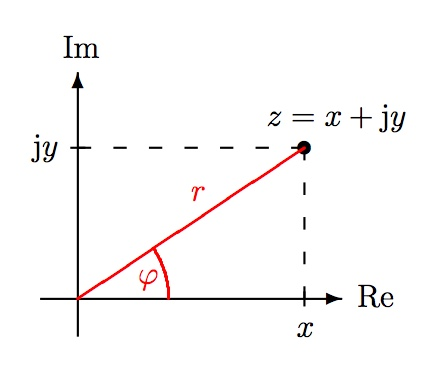
\includegraphics[width=3in]{kap6/komplexezahlen4}

\begin{Bemerkung}
Erinnerung\\
\end{Bemerkung}

Zusammenhang zwischen den Koordinaten $P(x,y)$ und $P(r,\varphi)$ :\\

$
\begin{pmatrix}
x=r*cos(\varphi)\\
\\
y=r*sin(\varphi)
\end{pmatrix}
$
bzw.
$
\begin{pmatrix}
r= \sqrt{x^2+y^2}\\
\\
tan(\varphi) = \frac{y}{x}
\end{pmatrix}
$
\\
\\

\begin{Bemerkung}
Bemerkung\\
\end{Bemerkung}

Der Zusammenhang zwischen dem Quotienten $\frac{x}{y}$ und dem Winkel $\varphi \in [0,2\pi)$ eindeutig, da die Tangensfunktion -periodisch ist.\\
Damit erhält man die \textbf{trigonometrische Darstellung} :\\

$z=x+j*y =r*cos(\varphi)+j*r*sin(\varphi) \Rightarrow z=r(cos(\varphi)+j*sin(\varphi))$\\

Dieser Ausdruck von $z$ wird im Folgenden sehr h"aufig auftreten. Deshalb wird daf"ur die Abk"urzung\\
\\
$e^{j\varphi} =cos(\varphi)+j*sin(\varphi)$\\
\\
ein.
Somit ergibt sich schließlich eine sehr kompakte Darstellung, die sogenannte \textbf{Exponentialdarstellung} einer komplexen Zahl:\\\\
$z=  {r(cos(\varphi)+r*j*sin(\varphi))}=r*e^{j\varphi}$

\begin{Bemerkung}
Zusammenfassung\\
\end{Bemerkung}

Eine komplexe Zahl l"asst sich auf verschiedene Arten darstellen:\\


\begin{tcolorbox}

\begin{enumerate}

\item $z=x+j*y$ (kartesische Darstellung)
\item $z=(cos(\varphi)+j*sin(\varphi))$ (trigonometrische Darstellung)
\item $z=r*e^{j\varphi}$ (Exponential-Darstellung)\\

\end{enumerate}

\end{tcolorbox}

	\subsection{Umrechnung zwischen den Darstellungen}
